\documentclass{report}
\usepackage[utf8]{inputenc}
\usepackage[italian]{babel}
\usepackage[T1]{fontenc}
\usepackage{tgpagella}
\usepackage{minted}
\title{
    Gym Manager \\
    \large Applicazioni e Servizi Web
}

\author{Claudia Giannelli - 001132530 \{claudia.giannelli2@studio.unibo.it\}\\
        Michele Ravaioli - 001136789 \{michele.ravaioli3@studio.unibo.it\}\\
        Eugenio Tampieri - 001125222 \{eugenio.tampieri@studio.unibo.it\}}

\usepackage{natbib}
\usepackage{graphicx}

\begin{document}

\maketitle
\section{Introduzione}
\par Il Gym Manager è una piattaforma progettata per facilitare la gestione delle attività di una palestra, consentendo ad amministratori, segretari, personal trainer e clienti di gestire i profili utente, calendari dei corsi della palestra e le prenotazioni ai corsi e alle sessioni private e in modo efficiente.
\par L'interazione iniziale avviene attraverso un amministratore, che configura il sistema aggiungendo i segretari, i personal trainer, i clienti e definendo i corsi disponibili. Gli amministratori hanno pieno controllo sulla gestione degli utenti e corsi, sulla loro modifica e cancellazione.
\par I segretari possono compiere le stesse operazioni degli amministratori, tranne aggiungere e visualizzare altri segretari o amministratori.
\par Ogni personal trainer dispone di un'area riservata dove può visualizzare i corsi che tiene e le sessioni private prenotate dai clienti. Inoltre, ha accesso ai dati dei clienti che sono iscritti ai corsi e alle sessioni private.
\par I clienti accedono alla loro area privata per visualizzare i propri dati personali, prenotare corsi o sessioni private, verificando la disponibilità dei trainer e, se necessario, cancellare una prenotazione. In caso di cancellazione da un corso il posto tornerà disponibile per altri utenti. I clienti non possono iscriversi a corsi già al completo o prenotare lezioni private già assegnate ad altri utenti.
\par Per migliorare la comunicazione tra gli utenti, il sistema integra una chat di assistenza in tempo reale, che consente ai clienti e ai personal trainer di contattare direttamente un amministratore per ricevere supporto su prenotazioni, corsi e altre richieste. Questa funzionalità è gestita tramite Socket.IO, che permette lo scambio immediato di messaggi tra utenti, garantendo un'interazione fluida e veloce.
\section{Requisiti}
\subsection{Requisiti non funzionali}
\par Come requisito fondamentale del progetto è richiesto lo sviluppo dell'applicazione utilizzando lo stack MEVN, e quindi la creazione di una single-page application basata su:
\begin{itemize}
    \item MongoDB per la persistenza;
    \item Express per il backend e le API;
    \item Vue.js come framework per lo sviluppo frontend; 
    \item Node.js per il runtime del server;
\end{itemize}
\par Come altri requisiti non funzionali, si sono individuati i seguenti quality attributes:
\begin{itemize}
    \item \textbf{Usabilità}: il sistema deve offrire un'interfaccia intuitiva e semplice da usare per tutti gli utenti, e l'accesso alle diverse funzionalità deve essere chiaro e ben organizzato.
    \item \textbf{Sicurezza}: ogni utente deve avere credenziali di accesso univoche e protette. Gli utenti devono poter accedere solo alle funzionalità permesse dal loro ruolo.
\end{itemize}
\subsection{Requisiti funzionali}
\par Le funzionalità richieste sono le seguenti, raggruppate per ruolo dell'utente:
\subsubsection{Amministratori}
\par Gli amministratori hanno il controllo completo del sistema e possono eseguire le seguenti operazioni:
\begin{itemize}
    \item Effettuare il login nel sistema.
    \item Registrare e salvare i profili dei clienti nel database.
    \item Registrare e salvare i profili dei personal trainer nel database.
    \item Registrare e salvare i profili dei segretari nel database.
    \item Creare nuovi corsi e gestire i dettagli dei corsi.
    \item Modificare i dettagli dei corsi, i profili dei clienti, i profili dei personal trainer e i profili dei segretari.
    \item Eliminare corsi, profili dei clienti e profili dei personal trainer.
    \item Aggiungere e gestire i segretari.
    \item Gestire le prenotazioni ai corsi e alle sessioni private.
    \item Fornire supporto agli utenti tramite la chat di assistenza in tempo reale.
    \item Accedere ai profili degli utenti (trainer e clienti) ed effettuare operazioni in loro vece.
\end{itemize}
\subsubsection{Segretari}
\par I segretari possono gestire il sistema esattamente come gli amministratori, con alcune limitazioni:
\begin{itemize}
    \item Non possono aggiungere o gestire altri segretari o amministratori.
    \item Non possono modificare direttamente i propri dati, ma devono richiedere eventuali modifiche all'amministratore.
\end{itemize}
\subsubsection{Personal Trainer}
\par I personal trainer hanno accesso a una loro area riservata con le seguenti funzionalità:
\begin{itemize}
    \item Effettuare il login per accedere ai propri dati personali e al calendario degli appuntamenti.
    \item Visualizzare l'elenco dei corsi che insegnano.
    \item Visualizzare l'elenco delle sessioni private prenotate con loro.
    \item Visualizzare i dettagli di un corso e la lista dei partecipanti iscritti.
    \item Visualizzare i dettagli dei partecipanti ai corsi e alle sessioni private.
    \item Contattare un amministratore per assistenza tramite la chat in tempo reale.
    \item Non possono modificare direttamente i propri dati, ma devono richiedere eventuali modifiche all'amministratore.
\end{itemize}
\subsubsection{Clienti}
\par I clienti possono interagire con il sistema per gestire le loro prenotazioni:
\begin{itemize}
    \item Effettuare il login per visualizzare il proprio profilo e le prenotazioni attive.
    \item Annullare l'iscrizione a un corso o a una sessione privata, liberando il posto per altri utenti.
    \item Visualizzare e iscriversi ai corsi disponibili (se un corso è completo, non possono iscriversi).
    \item Prenotare sessioni private selezionando un personal trainer e una fascia oraria disponibile.
    \item Non possono modificare direttamente i propri dati, ma devono richiedere eventuali modifiche all'amministratore.
    \item Contattare un amministratore per assistenza tramite la chat in tempo reale.
\end{itemize}
\section{Design}
\par Il sistema, realizzato sullo stack MEVN, si compone di una single-page application per il frontend e di un backend che fornisce le API REST \citep{rest} necessarie al funzionamento della SPA. La divisione in due componenti permette sia una maggiore scalabilità, che un miglior riuso del codice.
\subsection{Design del backend}
\par Il backend è stato progettato per fornire operazioni CRUD autenticate sulle varie entità del dominio applicativo tramite API REST. Nello specifico, le operazioni sulle entità sono le seguenti:
\begin{description}
    \item[Course (corso)] creazione, lista, recupero tramite ID, aggiornamento, eliminazione e lista, aggiunta ed eliminazione di una prenotazione.
    \item[Session (sessione con un personal trainer)] creazione, lista, recupero tramite ID ed eliminazione.
    \item[Customer (cliente della palestra)] creazione, lista, recupero tramite ID, aggiornamento ed eliminazione; lista delle prenotazioni e delle sessioni.
    \item[Trainer (istruttore o personal trainer)] creazione, lista, recupero tramite ID, aggiornamento ed eliminazione; lista delle prenotazioni e delle sessioni.
    \item[Admin (segretari o amministratori)] creazione, lista, recupero tramite ID, modifica ed eliminazione.
\end{description}
\par In più, il backend gestisce la parte di comunicazione real time per gli aggiornamenti delle entità e le chat.
\subsection{Design del frontend}
\par Si è scelto di procedere ad un approccio mobile first, con una particolare attenzione ai casi in cui la maggiore larghezza dello schermo possa essere utilizzata per presentare più informazioni contemporaneamente. Per semplificare la fase di progettazione, sono stati realizzati mockup dell'interfaccia.
\par Inoltre, sono stati considerati i seguenti aspetti durante la fase di progettazione:
\begin{itemize}
    \item Adottare un design inclusivo che consenta agli utenti di effettuare le stesse operazioni, a prescindere dal viewport
    \item Mostrare all'utente il risultato delle operazioni compiute tramite l'invio di notifiche
    \item Inviare modals di conferma per operazioni potenzialmente pericolose
    \item Progettare l'interfaccia in modo che le interazioni siano corte ed il risultato sia quindi ottenibile facilmente
    \item Visualizzare in modo ben evidente il titolo della pagina ed un pulsante per tornare indietro
    \item Adottare un'estetica minimalista, che consenta all'utente di focalizzarsi sul contenuto e sulle operazioni da svolgere
    \item Utilizzo di elementi visivi consistenti, in modo da sfruttare il linguaggio simbolico e delle metafore per facilitare le interazioni
    \item Utilizzo di accenti, colori ed icone (quest'ultimo ove effettivamente necessario) per rendere più chiara l'interfaccia
\end{itemize}
\par L'interfaccia è strutturata in diverse pagine, ognuna dedicata a una specifica operazione dell'utente.
\subsubsection{Accesso e autenticazione}
\par All'apertura dell'applicazione, l'utente visualizza la pagina di login, che consente l'autenticazione e il reindirizzamento alla pagina principale in base al ruolo assegnato. Dopo l'accesso, ogni utente può consultare la propria pagina profilo, dove sono riportate le informazioni personali e dove è possibile effettuare il logout.
\subsubsection{Interfaccia per i clienti}
\begin{figure}[h!]
    \centering
    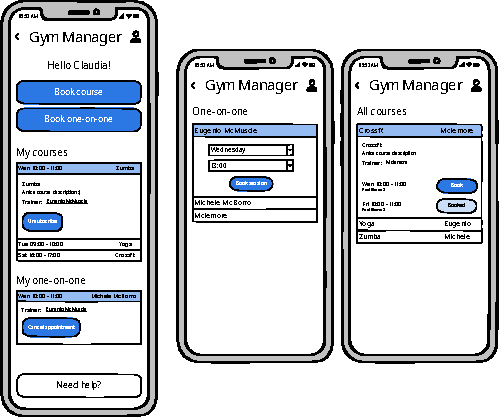
\includegraphics[scale=1.5]{user-mockups.pdf}
    \caption{Mock up clienti}
    \label{fig:deathstar}
\end{figure}
    
\par La pagina principale dei clienti mostra:
\begin{itemize}
    \item I corsi a cui sono iscritti, con dettagli come descrizione, trainer e orari.
    \item Le sessioni private prenotate con i trainer.
\end{itemize}
\par Da qui, i clienti possono annullare le iscrizioni ai corsi o alle sessioni prenotate. Inoltre, sono presenti due pulsanti che permettono di:
\begin{itemize}
    \item Iscriversi a un nuovo corso.
    \item Prenotare una sessione privata con un trainer.
\end{itemize}
\par Nella pagina di registrazione ai corsi, vengono elencati tutti i corsi disponibili in palestra, permettendo agli utenti di selezionare una fascia oraria per l'iscrizione.
\par La pagina di prenotazione delle sessioni mostra invece l'elenco dei trainer, consentendo la selezione di un giorno e un orario per richiedere una sessione privata.
\subsubsection{Interfaccia per i trainer}
\begin{figure}[h!]
    \centering
    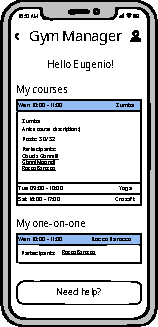
\includegraphics[scale=1.5]{trainer-mockups.pdf}
    \caption{Mock up trainer}
    \label{fig:deathstar}
\end{figure}
\par La pagina principale dei trainer contiene:
\begin{itemize}
    \item L'elenco dei corsi, con descrizione e partecipanti, di cui sono istruttori.
    \item Le sessioni private prenotate dagli utenti.
\end{itemize}
\subsubsection{Interfaccia per gli amministratori}
\begin{figure}[h!]
    \centering
    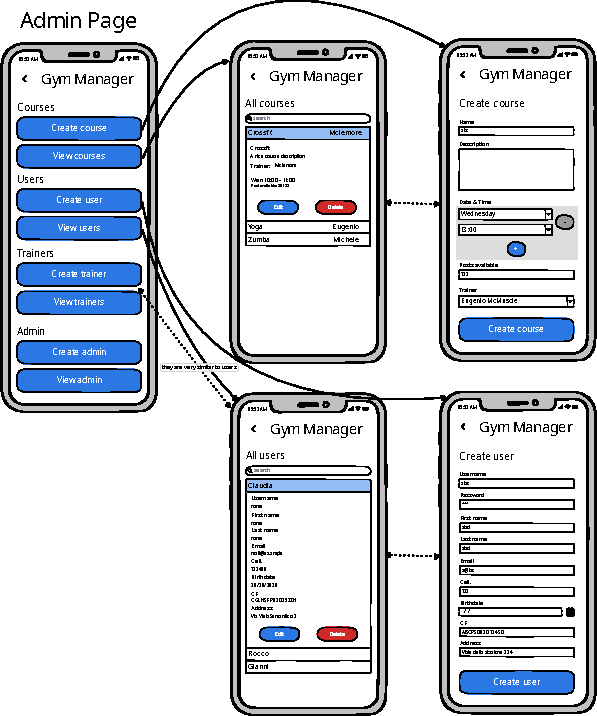
\includegraphics[scale=1]{admin-mockups.pdf}
    \caption{Mock up trainer}
    \label{fig:deathstar}
\end{figure}
\par Gli amministratori hanno accesso a una pagina che consente la gestione completa della palestra, includendo le seguenti operazioni:
\begin{itemize}
    \item Visualizzazione della lista completa degli utenti, con la possibilità di modificarli o eliminarli.
    \item Creazione di nuovi utenti attraverso un apposito form.
\end{itemize}
\par L'accesso alle diverse funzioni avviene tramite pulsanti che indirizzano l'admin alle pagine dedicate.
\subsubsection{Interfaccia per i segretari}
\par La pagina dei segretari è identica a quella degli amministratori, con l'unica eccezione che non include le operazioni relative alla gestione degli amministratori.

\section{Tecnologie}
\par Il sistema è stato sviluppato con un'architettura composta da un frontend reattivo, un backend basato su Node.js, un database NoSQL per la gestione dei dati e un sistema di comunicazione in tempo reale. Inoltre, l'uso di Docker garantisce portabilità e coerenza degli ambienti di sviluppo e produzione.
\par Le interfacce utente sono state realizzate utilizzando il framework Bootstrap e, dove necessario per rendere l'interfaccia più chiara, le icone FontAwesome.
\subsection{Frontend}
\par Il frontend è stato sviluppato utilizzando HTML, CSS, TypeScript, Vue.js e Socket.IO, fornendo un'interfaccia moderna, dinamica e altamente interattiva. Sono stati utilizzati anche i JSON Web Token \citep{rfc7519} per l'autenticazione, che contengono anche il profilo dell'utente, riducendo il numero di richieste necessarie.
\par È stato scelto di realizzare il frontend in TypeScript per la migliore integrazione con Vue.js e per l'esperienza di sviluppo ottenibile con un linguaggio tipato staticamente.
\par Si è inoltre fatto ampio uso dei componenti di Vue.js, per aderire ai principii di separation of concerns e single responsibility principle.
\par È stato utilizzato Pinia per mantenere lo stato globale dell'applicazione e per fornire funzionalità globali quali l'invio di notifiche.
\subsection{Backend}
\par Il backend è stato sviluppato con Node.js e il framework Express.js.
\par Per la gestione della chat di assistenza, è stato integrato Socket.IO, che permette:
\begin{itemize}
    \item Connessione bidirezionale tra client e server senza necessità di aggiornare la pagina.
    \item Supporto ai WebSockets, con fallback su altre tecnologie (HTTP long polling) per garantire compatibilità.
    \item Notifiche in tempo reale per aggiornamenti sulle prenotazioni o messaggi di assistenza.
\end{itemize}
\par Per la gestione dei dati è stato scelto MongoDB, un database NoSQL altamente scalabile, e Mongoose, un Object Data Modeling (ODM) che consente di:
\begin{itemize}
    \item Definire schemi precisi per la struttura dei dati.
    \item Implementare validazioni e middleware per garantire l'integrità dei dati.
    \item Supportare operazioni avanzate come popolazione dei dati e query complesse.
\end{itemize}
\par L'utilizzo dei JWT (grazie alla libreria jose)  consente di gestire tramite un semplice middleware l'autenticazione, senza dover tener traccia delle sessioni.
\par Le password vengono memorizzate \textit{salted and hashed} con l'algoritmo Argon2id\citep{rfc9106}, considerato stato dell'arte in quanto computazionalmente complesso da invertire, anche con l'ausilio di GPU.
\section{Codice}
\par Di seguito verranno mostrati quattro esempi che ci sembrano esemplificare la natura del progetto e ci permettono di motivare le nostre scelte tecniche.
\subsection{\texttt{ValidatingGenericInput}}
\begin{minted}{html}
<script setup lang="ts">
import { computed } from 'vue';
const props = defineProps<{
    validationFunction: (value: string) => boolean,
    errorMessage: string,
    type: string,
    id: string,
    dontAutocapitalize?: boolean,
}>();
const model = defineModel<string>(); 
const validationModel = defineModel<boolean>("valid");

const fieldValid = computed(() => {
    const status = props.validationFunction(model.value || "");
    validationModel.value = status;
    return status;
});

const class = computed(() => `form-control ${
    ((model?.length || 0 > 0) && errorMessage.length > 0) ?
    (fieldValid ? 'is-valid' : 'is-invalid') : ''}`);

</script>
<template>
    <div class="mb-3">
        <label class="form-label" :for="id">
            <slot></slot>
        </label>
        <input ref="input" :aria-invalid="!fieldValid"
            required aria-required="true"
            :class="class"
            :type="type" :id="id" v-model="model"
            :autocapitalize="dontAutocapitalize ? 'none' : 'yes'">
        <div class="invalid-feedback">{{ props.errorMessage }}</div>
    </div>
</template>
\end{minted}
\par Questo componente è stato scelto perché mostra le potenzialità di Vue nell'incapsulazione e nella reattività.
\subsubsection{\texttt{CourseAvailabilityWatcher}}
\begin{minted}{html}
    <script setup lang="ts">
import { io } from 'socket.io-client';
import { EventType, SubscriptionEntity } from '@gym-manager/models';
import { useUserStore } from '@/store/user';
import { onMounted } from 'vue';

export interface CourseAvailabilityUpdate {
    course: string,
    availability: number,
    dayOfWeek: string,
    startTime: string,
}

const emit = defineEmits<{ update: [CourseAvailabilityUpdate] }>();

const client = useUserStore().client;
const socket = io({
    path: "/api/socketio",
});

onMounted(() => {
    socket.emit(EventType.Subscribe.toString(), {
        token: client.authToken!,
        entity: SubscriptionEntity.CourseAvailability
    });
});

socket.on(
    EventType.SubscriptionUpdate.toString(),
    (u: CourseAvailabilityUpdate) => emit('update', u)
);

</script>
<template>
</template>
\end{minted}
\par Qui si può notare l'utilizzo delle interfacce per la definizione dei messaggi emessi, ma soprattutto la comodità di incapsulare elementi interattivi di terze parti in componenti Vue, per integrarli con la reattività.
\subsection{\texttt{fetchCourseBy\_Id}}
\begin{minted}{js}
    static async fetchCourseBy_Id(req, res) {
        console.log("fetchCourseBy_Id");
        const id = req.params.id;
        try {
            const course = await Course.findById(id, idProjection(Course), null)
                .exec();
            res.status(200).json(course);
        } catch (error) {
            res.status(404).json({ message: error.message });
        } finally {
        }
    }
\end{minted}
\par Questo è uno dei tanti metodi dell'API, e mostra come sia facile integrare MongoDB con Express per fornire i documenti tramite una API REST.
\par Si noti anche l'utilizzo delle risposte HTTP \citep{rfc2616}.
\subsubsection{\texttt{createAuthMiddleware}}
\begin{minted}{js}
const createAuthMiddleware = (roles) => async function authMiddleware(req, res, next) {
    if (req.headers["authorization"] !== undefined) {
        let jwt = req.headers["authorization"].split(' ')[1];
        const { payload, _ } = await verifyJWT(jwt);
        const jwt_payload = payload;
        if (jwt_payload.error === undefined && roles.has(parseRole(jwt_payload.role))) {
            // JWT is still valid
            req.user = jwt_payload.profile
            req.user.role = parseRole(jwt_payload.role);
        } else {
            res.contentType("text/plain")
                .status(401)
                .send(`Invalid token${jwt_payload.error === undefined ?
                    "" : ": " + jwt_payload.error.code}`);
            return;
        }
    }
    next();
};
\end{minted}
\par Questa è la funzione che crea i middleware utilizzati per proteggere gli endpoint dagli accessi non autorizzati. Qui è possibile notare come sia possibile separare i diversi aspetti della gesitione della richiesta (in questo caso l'autenticazione) in componenti diverse.
\section{Test}
\par Sono stati effettuati degli usability test per raccogliere feedback dall'utente tramite la metodologia del cognitive walkthrough. Durante i test sono emersi alcuni dettagli non considerati in fase di design, oltre ad alcuni errori negli edge case. A titolo esemplificativo, sono state apportate le seguenti modifiche:
\begin{itemize}
    \item spostamento dell'ordine dei campi
    \item feedback se non è online nessuno per rispondere alle chat
    \item ottimizzazione dei campi username per mobile
\end{itemize}
\section{Deployment}
\par Si è scelto di suddividere l'applicazione in due container: uno per il frontend e uno per il backend. Il container del frontend è un container NGINX configurato per servire solo il frontend.
\par Questa suddivisione permetterebbe di scalare in modo diverso frontend e backend. In questo progetto non si sono compiuti i test necessari a garantire il funzionamento di più backend in contemporanea, perché sarebbe stato necessario configurare Træfik per reindirizzare le richieste di Socket.IO sempre alla stessa istanza del backend. Inoltre, sarebbe opportuno utilizzare tecnologie come Redis per la memorizzazione dello stato necessario a gestire le chat. Altri benefici imputabili a questa architettura sono quelli di non far servire a Express il frontend e di poter aggiornare le due componenti in modo indipendente.
\par Inoltre, nella configurazione contenuta in docker-compose.yaml, viene utilizzato Træfik come reverse proxy e gateway per lo smistamento delle richieste al servizio corretto. Per questo i container contengono già le label per il setup automatico di Træfik.
\par Infine, sono state configurate le GitHub Actions per pubblicare automaticamente le immagini dell'applicazione ad ogni commit sul branch master.
\subsection{Istruzioni per il deployment}
\par Per eseguire in locale il progetto, è semplicemente necessario eseguire il seguente comando nella radice:
\begin{minted}{bash}
    docker compose build
    docker compose up
\end{minted}
\par Il frontend verrà avviato sulla porta 8080 (HTTP) e sarà possibile accedere con le credenziali \texttt{admin}/\texttt{admin}.
\section{Conclusioni}
\par Realizzare Gym Manager ci ha consentito di verificare come le moderne tecnologie web possano essere integrate per creare un'applicazione scalabile, efficiente e intuitiva e garantire un ottimo riuso del codice. Grazie all'adozione di un'architettura basata su Vue.js per il frontend, Node.js con Express.js per il backend e MongoDB come database, il sistema garantisce un'esperienza fluida e interattiva per amministratori, personal trainer e clienti.
\par Uno degli aspetti più rilevanti di questo progetto è l'uso di Vue.js come framework principale per il frontend. Vue.js è stato scelto per la sua reattività, modularità e semplicità di integrazione, permettendo di sviluppare un'interfaccia utente dinamica e altamente interattiva.
\par La suddivisione in package all'interno dello stesso workspace ha permesso di condividere del codice e garantirne la consistenza, come ad esempio i ruoli degli utenti e i tipi di messaggi inviati tramite Socket.IO.
\par Abbiamo potuto anche constatare i limiti di JavaScript per i progetti non di piccole dimensioni, e di come TypeScript faciliti lo sviluppo. Abbiamo però avuto anche l'impressione che TypeScript sia il cosiddetto glass of cold water in hell, in quanto non sempre è precisa la corrispondenza fra tipi del type system e tipi di dato.
\par Sul lato backend, Node.js con Express.js ha garantito un'architettura leggera e scalabile, con un'API RESTful ottimizzata per gestire le operazioni CRUD su utenti, corsi e prenotazioni. La scelta di MongoDB ha permesso di implementare un database flessibile e performante, in grado di gestire grandi volumi di dati senza compromettere le prestazioni.
\par Un altro aspetto fondamentale del progetto è stato l'uso di Socket.IO per la gestione della chat di assistenza in tempo reale, fornendo un canale diretto di comunicazione tra clienti, trainer e amministratori. Questo ha migliorato significativamente l'interazione tra gli utenti, offrendo un servizio di supporto immediato e riducendo i tempi di risposta.
\par In conclusione, il progetto ha raggiunto tutti gli obiettivi prefissati, fornendo una piattaforma robusta, scalabile e sicura per la gestione delle attività di una palestra.
\bibliographystyle{plain}
\bibliography{references}
\end{document}
